\section{eo\-VRPMutation Class Reference}
\label{classeo_v_r_p_mutation}\index{eoVRPMutation@{eoVRPMutation}}
Implementation of variations of the four mutation operators for the VRP-TW defined by Tavares et al.  


{\tt \#include $<$eo\-VRPMutation.h$>$}

Inheritance diagram for eo\-VRPMutation::\begin{figure}[H]
\begin{center}
\leavevmode
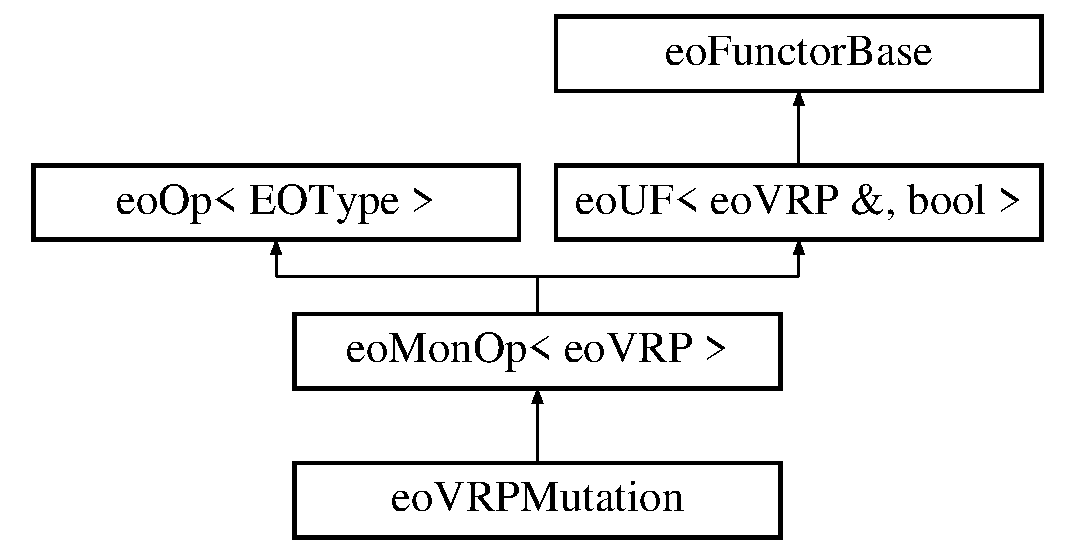
\includegraphics[height=4cm]{classeo_v_r_p_mutation}
\end{center}
\end{figure}
\subsection*{Public Member Functions}
\begin{CompactItemize}
\item 
\bf{eo\-VRPMutation} ()\label{classeo_v_r_p_mutation_419ac5c738369876de09212a844e67c3}

\begin{CompactList}\small\item\em Default constructor: nothing to do here. \item\end{CompactList}\item 
std::string \bf{class\-Name} () const 
\begin{CompactList}\small\item\em Returns a string containing the name of the class. \item\end{CompactList}\item 
bool \bf{operator()} (\bf{eo\-VRP} \&\_\-genotype)
\begin{CompactList}\small\item\em Functor operator. \item\end{CompactList}\end{CompactItemize}
\subsection*{Private Member Functions}
\begin{CompactItemize}
\item 
bool \bf{swap\-Mutation} (\bf{eo\-VRP} \&\_\-genotype)
\begin{CompactList}\small\item\em It exhanges the positions of two clients within the individual. \item\end{CompactList}\item 
bool \bf{inversion\-Mutation} (\bf{eo\-VRP} \&\_\-genotype)
\begin{CompactList}\small\item\em It selects two positions in the genotype and inverts the clients between them. \item\end{CompactList}\item 
bool \bf{insertion\-Mutation} (\bf{eo\-VRP} \&\_\-genotype)
\begin{CompactList}\small\item\em It selects and individual, erases it from its original position and inserts it somewhere else. \item\end{CompactList}\item 
bool \bf{Displacement\-Mutation} (\bf{eo\-VRP} \&\_\-genotype)
\begin{CompactList}\small\item\em It selects a set of clients, erases them from their original position and inserts them somewhere else. \item\end{CompactList}\end{CompactItemize}


\subsection{Detailed Description}
Implementation of variations of the four mutation operators for the VRP-TW defined by Tavares et al. 

These four operators should be separated in different classes and their probabilities made parameterizable. 



Definition at line 52 of file eo\-VRPMutation.h.

\subsection{Member Function Documentation}
\index{eoVRPMutation@{eo\-VRPMutation}!className@{className}}
\index{className@{className}!eoVRPMutation@{eo\-VRPMutation}}
\subsubsection{\setlength{\rightskip}{0pt plus 5cm}std::string eo\-VRPMutation::class\-Name (void) const\hspace{0.3cm}{\tt  [inline, virtual]}}\label{classeo_v_r_p_mutation_1c99e21818d6bae1cdd21b4180601d41}


Returns a string containing the name of the class. 

Used to display statistics. \begin{Desc}
\item[Returns:]The string containing the name of the class. \end{Desc}


Reimplemented from \bf{eo\-Mon\-Op$<$ eo\-VRP $>$}.

Definition at line 70 of file eo\-VRPMutation.h.\index{eoVRPMutation@{eo\-VRPMutation}!operator()@{operator()}}
\index{operator()@{operator()}!eoVRPMutation@{eo\-VRPMutation}}
\subsubsection{\setlength{\rightskip}{0pt plus 5cm}bool eo\-VRPMutation::operator() (\bf{eo\-VRP} \& {\em \_\-genotype})\hspace{0.3cm}{\tt  [inline, virtual]}}\label{classeo_v_r_p_mutation_f9fabdc8497f463add309fdace102813}


Functor operator. 

Applies one of the four mutation operators available, each of them with a predefined (hard-coded) probability. These operators should be separated in different classes and their probabilities made parameterizable to do it in a more \char`\"{}paradis\-EO\char`\"{} way. \begin{Desc}
\item[Parameters:]
\begin{description}
\item[{\em \_\-genotype}]The genotype being mutated (it will be probably modified). \end{description}
\end{Desc}
\begin{Desc}
\item[Returns:]True if the individual has been modified. False otherwise. \end{Desc}


Implements \bf{eo\-UF$<$ eo\-VRP \&, bool $>$}.

Definition at line 86 of file eo\-VRPMutation.h.

References eo\-VRP::clean\-Routes(), Displacement\-Mutation(), insertion\-Mutation(), inversion\-Mutation(), swap\-Mutation(), and eo\-Rng::uniform().\index{eoVRPMutation@{eo\-VRPMutation}!swapMutation@{swapMutation}}
\index{swapMutation@{swapMutation}!eoVRPMutation@{eo\-VRPMutation}}
\subsubsection{\setlength{\rightskip}{0pt plus 5cm}bool eo\-VRPMutation::swap\-Mutation (\bf{eo\-VRP} \& {\em \_\-genotype})\hspace{0.3cm}{\tt  [inline, private]}}\label{classeo_v_r_p_mutation_bef9736583de0b7f6e734b26483ab69d}


It exhanges the positions of two clients within the individual. 

Clients may or may not be in the same route. \begin{Desc}
\item[Parameters:]
\begin{description}
\item[{\em \_\-genotype}]The genotype being mutated (it will be probably modified). \end{description}
\end{Desc}
\begin{Desc}
\item[Returns:]True if the individual has been modified. False otherwise. \end{Desc}


Definition at line 119 of file eo\-VRPMutation.h.

References eo\-Rng::random().

Referenced by operator()().\index{eoVRPMutation@{eo\-VRPMutation}!inversionMutation@{inversionMutation}}
\index{inversionMutation@{inversionMutation}!eoVRPMutation@{eo\-VRPMutation}}
\subsubsection{\setlength{\rightskip}{0pt plus 5cm}bool eo\-VRPMutation::inversion\-Mutation (\bf{eo\-VRP} \& {\em \_\-genotype})\hspace{0.3cm}{\tt  [inline, private]}}\label{classeo_v_r_p_mutation_61cc39a190e9d070b005a7afb5e38d2a}


It selects two positions in the genotype and inverts the clients between them. 

Clients may or may not be in the same route. \begin{Desc}
\item[Parameters:]
\begin{description}
\item[{\em \_\-genotype}]The genotype being mutated (it will be probably modified). \end{description}
\end{Desc}
\begin{Desc}
\item[Returns:]True if the individual has been modified. False otherwise. \end{Desc}


Definition at line 142 of file eo\-VRPMutation.h.

References eo\-Rng::random().

Referenced by operator()().\index{eoVRPMutation@{eo\-VRPMutation}!insertionMutation@{insertionMutation}}
\index{insertionMutation@{insertionMutation}!eoVRPMutation@{eo\-VRPMutation}}
\subsubsection{\setlength{\rightskip}{0pt plus 5cm}bool eo\-VRPMutation::insertion\-Mutation (\bf{eo\-VRP} \& {\em \_\-genotype})\hspace{0.3cm}{\tt  [inline, private]}}\label{classeo_v_r_p_mutation_6ead0938bb1f8ab34c321916a6dd5b66}


It selects and individual, erases it from its original position and inserts it somewhere else. 

The insertion may or may not be within the same route. \begin{Desc}
\item[Parameters:]
\begin{description}
\item[{\em \_\-genotype}]The genotype being mutated (it will be probably modified). \end{description}
\end{Desc}
\begin{Desc}
\item[Returns:]True if the individual has been modified. False otherwise. \end{Desc}


Definition at line 170 of file eo\-VRPMutation.h.

References eo\-Rng::random().

Referenced by operator()().\index{eoVRPMutation@{eo\-VRPMutation}!DisplacementMutation@{DisplacementMutation}}
\index{DisplacementMutation@{DisplacementMutation}!eoVRPMutation@{eo\-VRPMutation}}
\subsubsection{\setlength{\rightskip}{0pt plus 5cm}bool eo\-VRPMutation::Displacement\-Mutation (\bf{eo\-VRP} \& {\em \_\-genotype})\hspace{0.3cm}{\tt  [inline, private]}}\label{classeo_v_r_p_mutation_b6b7e818085f6ba03d64f045f32356be}


It selects a set of clients, erases them from their original position and inserts them somewhere else. 

The selected set of clients may cover different routes. \begin{Desc}
\item[Parameters:]
\begin{description}
\item[{\em \_\-genotype}]The genotype being mutated (it will be probably modified). \end{description}
\end{Desc}
\begin{Desc}
\item[Returns:]True if the individual has been modified. False otherwise. \end{Desc}


Definition at line 199 of file eo\-VRPMutation.h.

References eo\-Rng::random().

Referenced by operator()().

The documentation for this class was generated from the following file:\begin{CompactItemize}
\item 
eo\-VRPMutation.h\end{CompactItemize}
